\chapter{System Design}
\section{Login and Authentication flow}
From our research, like looking at Snapchat which has some similarities to our project (login and camera functionalities) we understood that we had a good template to reference as to how our project should be structured. Snapchat (and most mobile applications) have the same screen stack. The first page a user who has not signed in before should see a screen that allows them to either sign in, create an account or reset their password. We decided that the user needs an entry box for both the username and password and then buttons for the other functionality on the screen. From here the user has options to do everything they need. We also wanted to include that app title on the page. 
\begin{center}
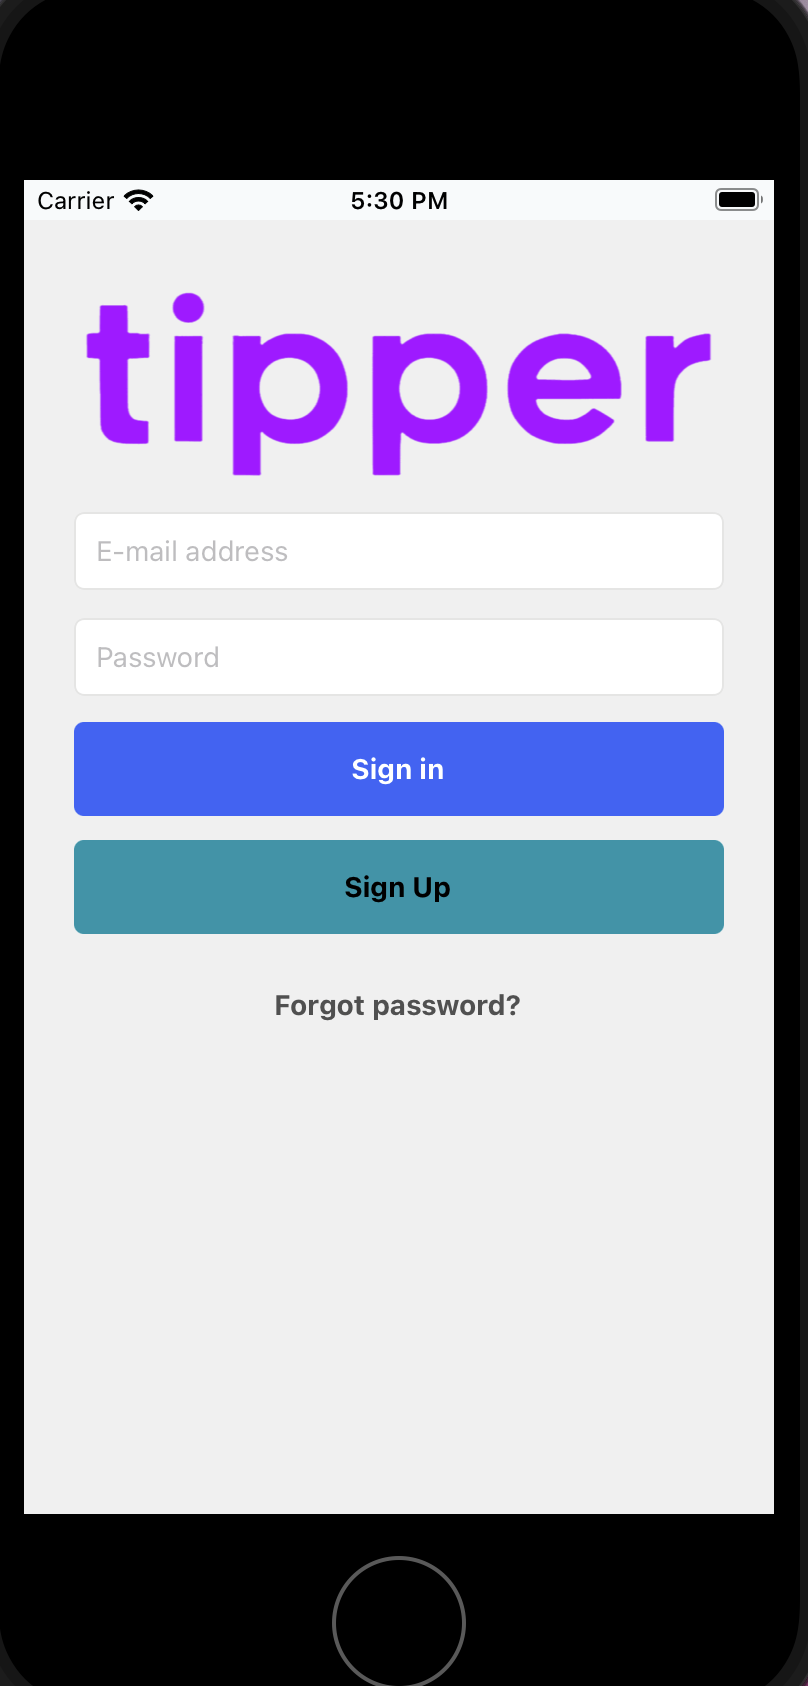
\includegraphics[scale = .40]{atu-computing-latex-template/images/SignInScreen.png}
\end{center}
When the user wants to create an account, they must tap the 'Sign Up' button. From there they are presented with two buttons. Either to sign up as a customer or an employee of a business. If the user decides to sign up as a customer, they are presented with input boxes for First Name, Second Name, Email Address, Phone Number and Password. The phone number isn't used for any authentication but keeps in line with the ability future additions to the app. The password has to include an uppercase, lowercase, a number and be at least eight characters in length.
\begin{center}
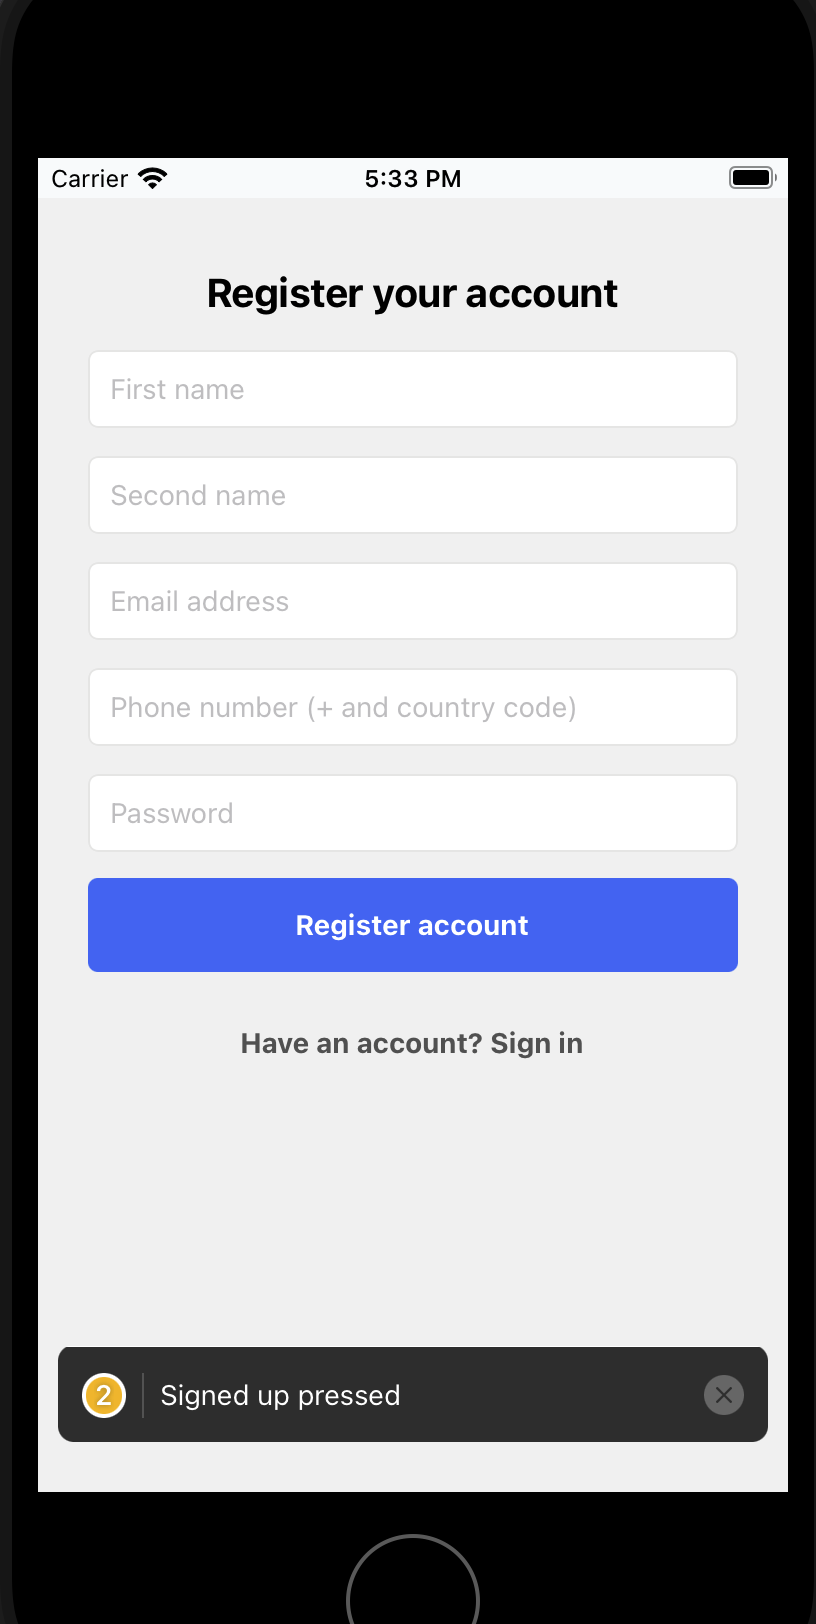
\includegraphics[scale = .40]{atu-computing-latex-template/images/SignUpCustomer.png}
\end{center}
Then the user must press register account button to be brought to a page where they must enter a verification code that is sent to them via email (one of the methods provided by AWS Amplify) and can get the code resent them via email again which is another methods provided. If pressed, this makes the previous verification code invalid. Once the valid code is entered, the user is then automatically brought back to the sign in screen. 
\begin{center}
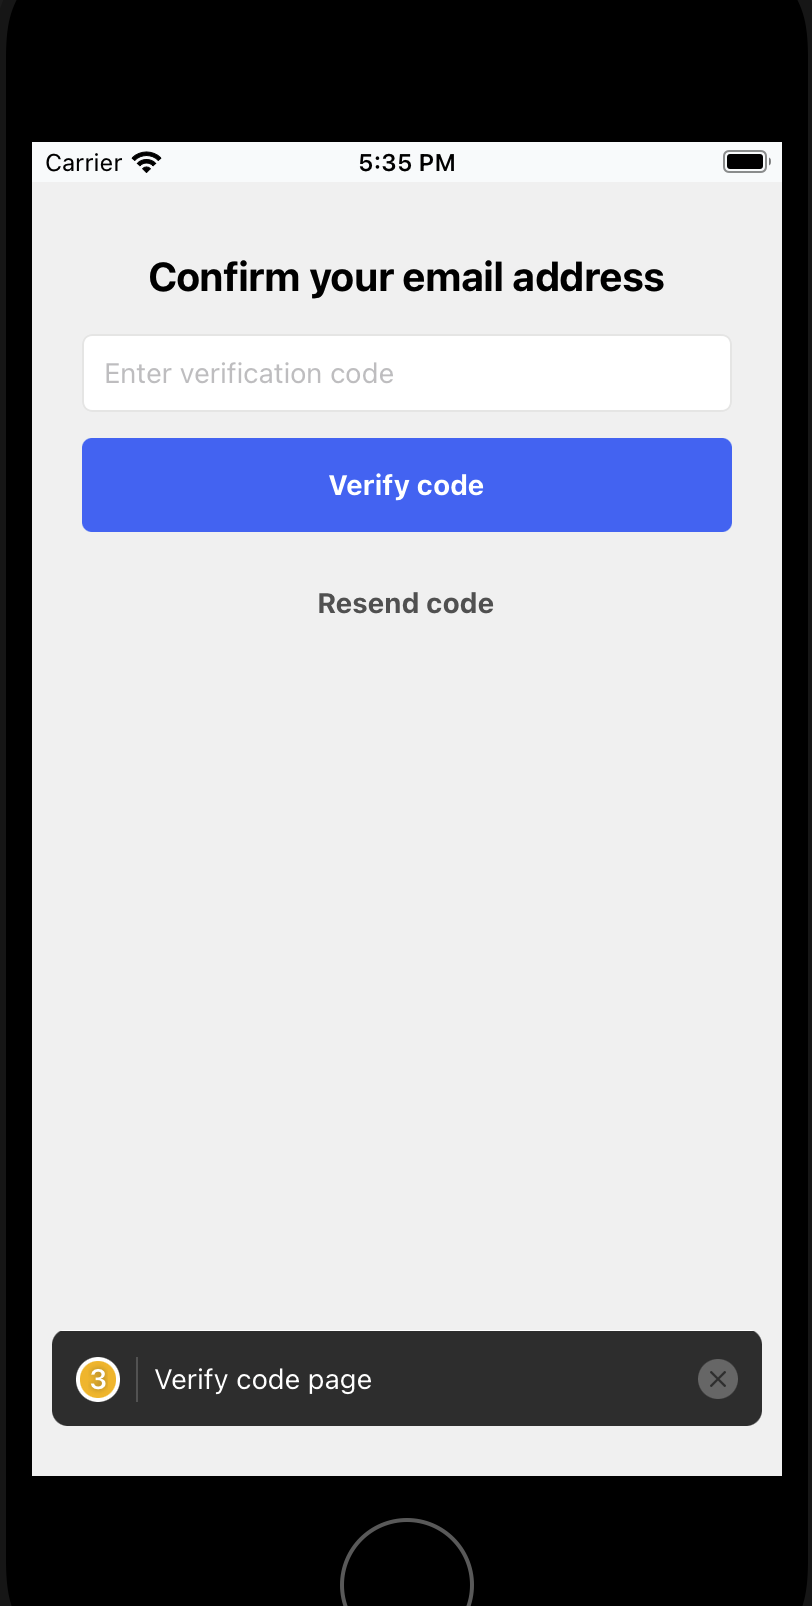
\includegraphics[scale = .40]{atu-computing-latex-template/images/ConfirmEmailCode.png}
\end{center}
On the other hand, if the user wants to sign up as an employee, the sign up process is slightly different. The entry boxes are the same as the customer sign up flow with the same button functionality. 
\begin{center}
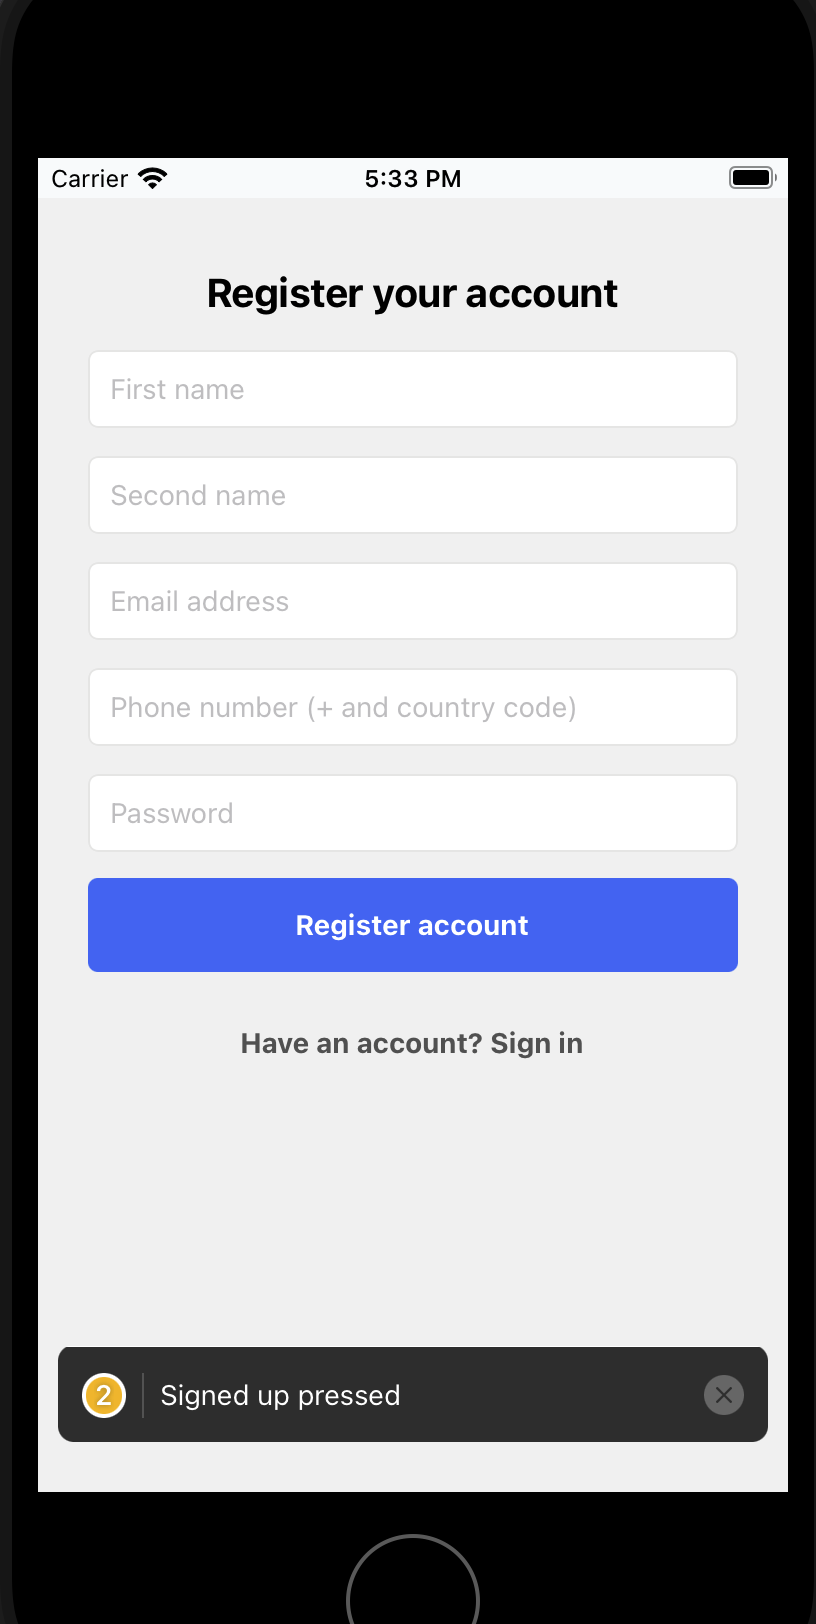
\includegraphics[scale = .30]{atu-computing-latex-template/images/SignUpCustomer.png}
\end{center}
They are then asked to enter the verification code and when the user has entered a valid verification code,
\begin{center}
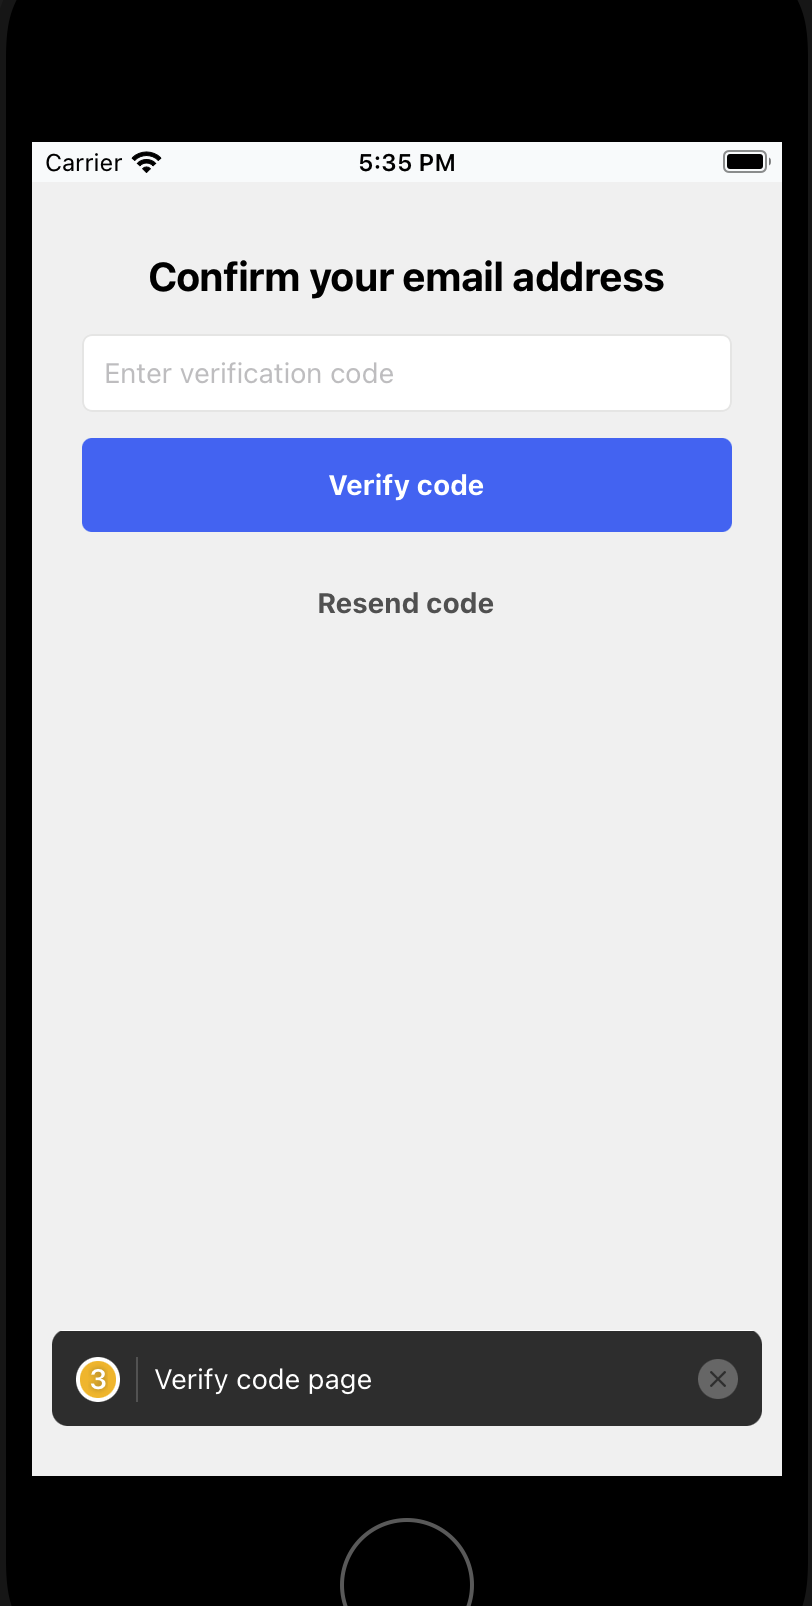
\includegraphics[scale = .40]{atu-computing-latex-template/images/ConfirmEmailCode.png}
\end{center}
The user is then brought to the QR Code generation screen. From here the user can enter their IBAN and hit a button to generate their unique QR code. They user can keep generating another QR code if they make a mistake. On this page the user also has the option to either save the QR code to their device, although this requires permission from the user to do this. The user can also send their QR code to the email address that they used when creating their account. Both of this happens when the respective button is pressed. After the user is happy, they hit the finish button to return back to the sign in screen. 
\begin{center}
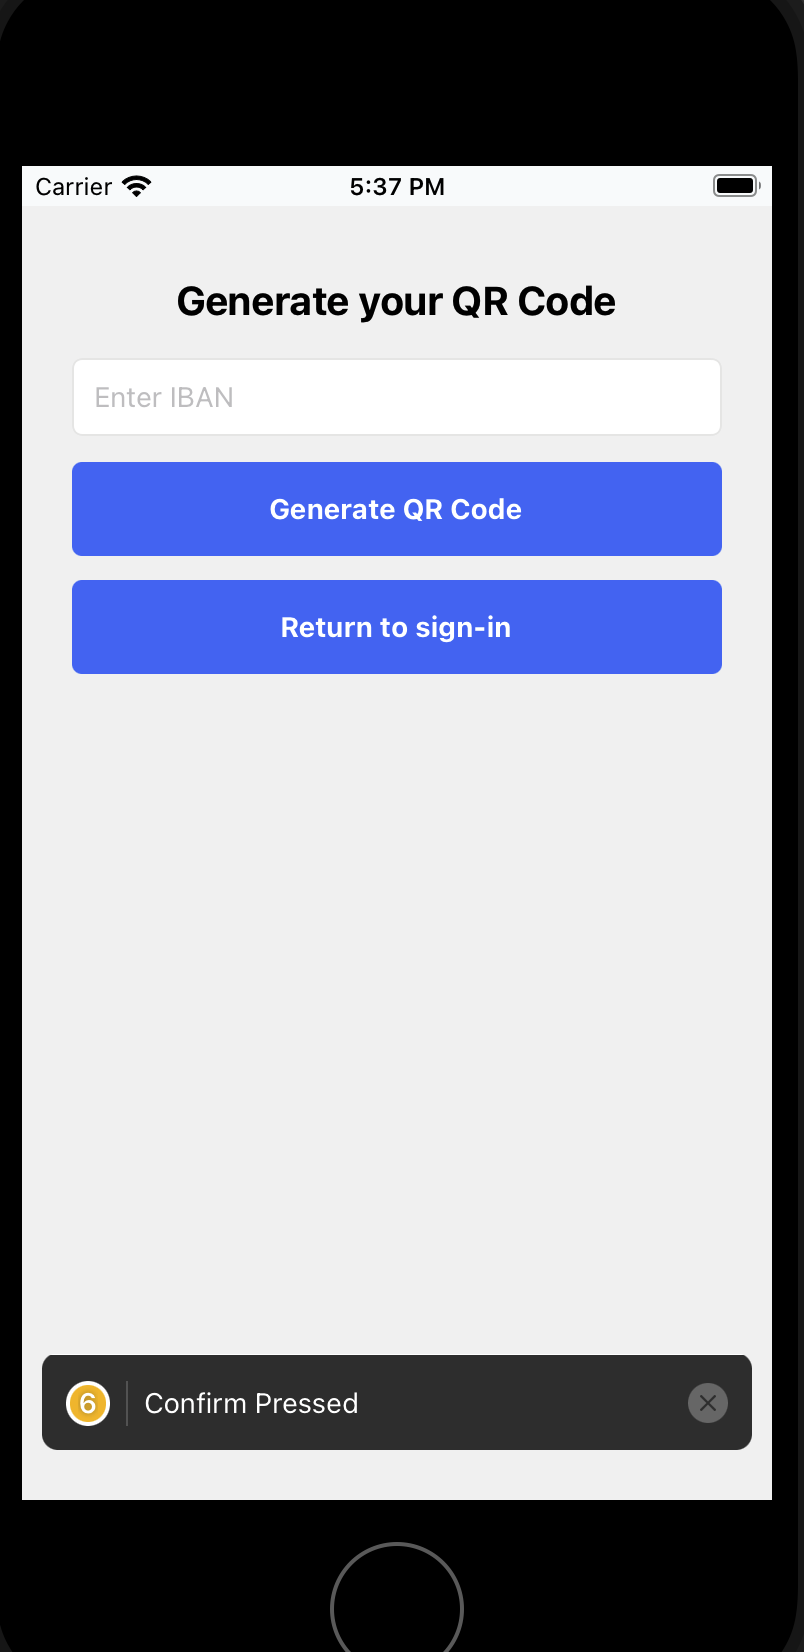
\includegraphics[scale = .40]{atu-computing-latex-template/images/GenerateQRCode.png}
\end{center}
Finally, on the sign in page is the option to reset their password by pressing the forgot password button. From here the user is asked to enter a valid email address of the account they would like to reset their password for. On this page the user presses a button to progress and is sent a verification code. 
\begin{center}
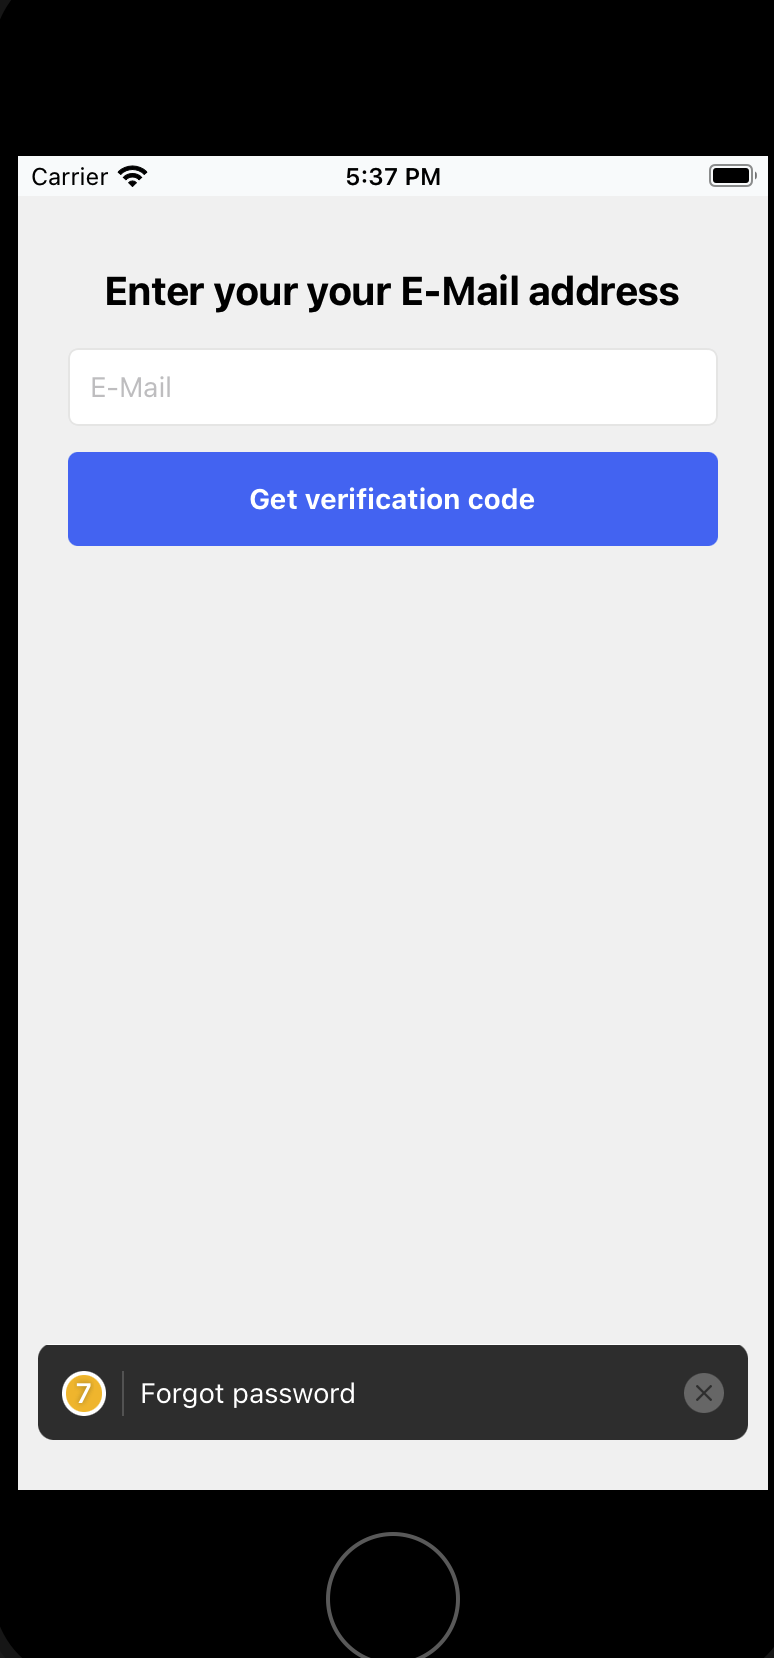
\includegraphics[scale = .40]{atu-computing-latex-template/images/EnterEmailReset.png}
\end{center}
On the next screen the user must enter a valid verification code that has been sent to their email address and the new password. The user can also request a new verification code as well. Once the verification code and password requirements have been met, the user will returned to the sign in page.
\begin{center}
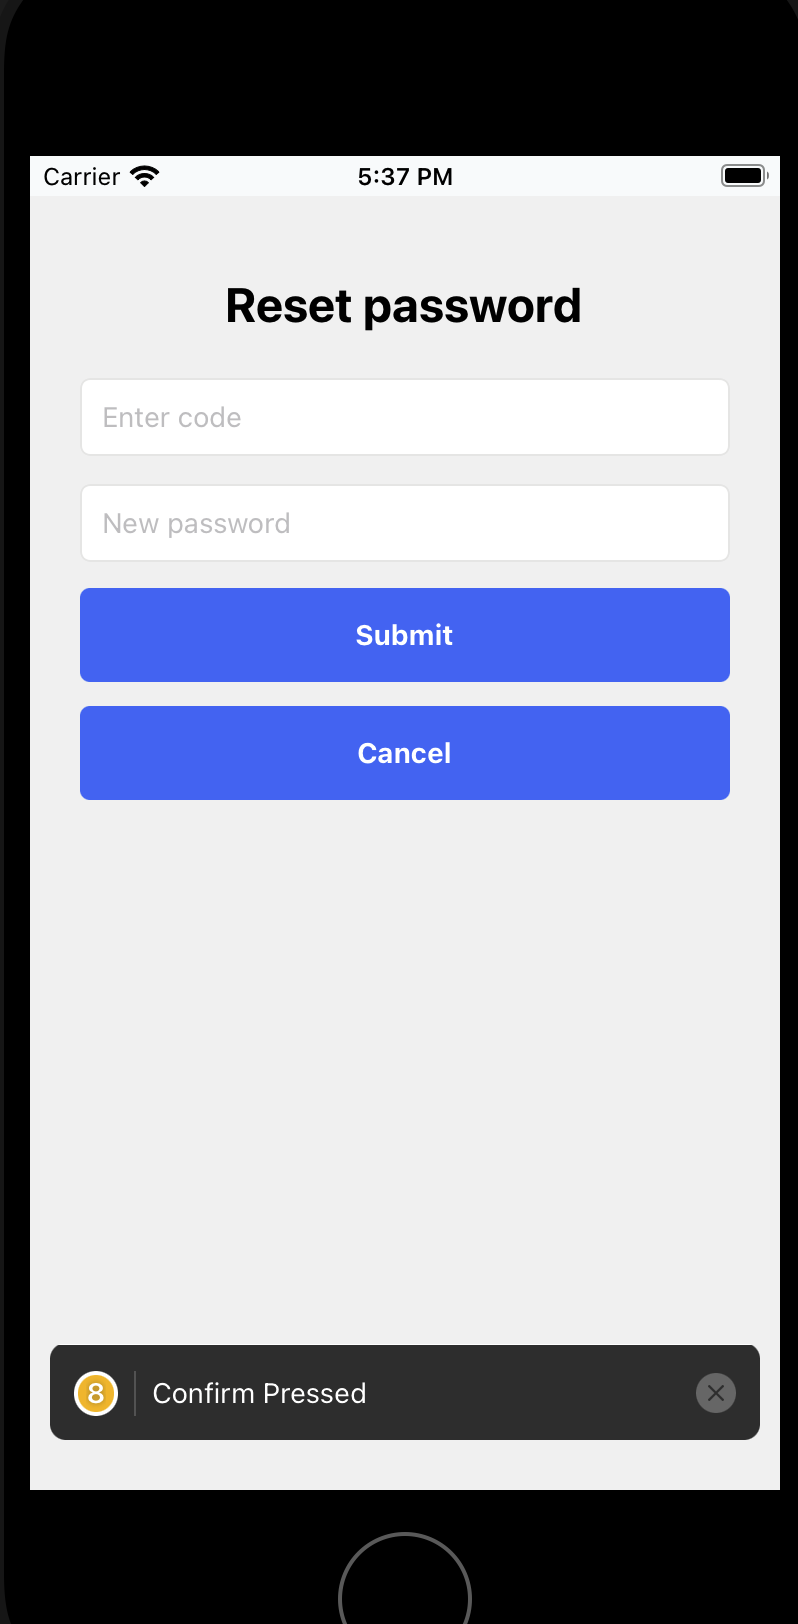
\includegraphics[scale = .40]{atu-computing-latex-template/images/EnterNewPassword.png}
\end{center}
Here is a complete UML diagram showing the entire authentication flow
\begin{center}
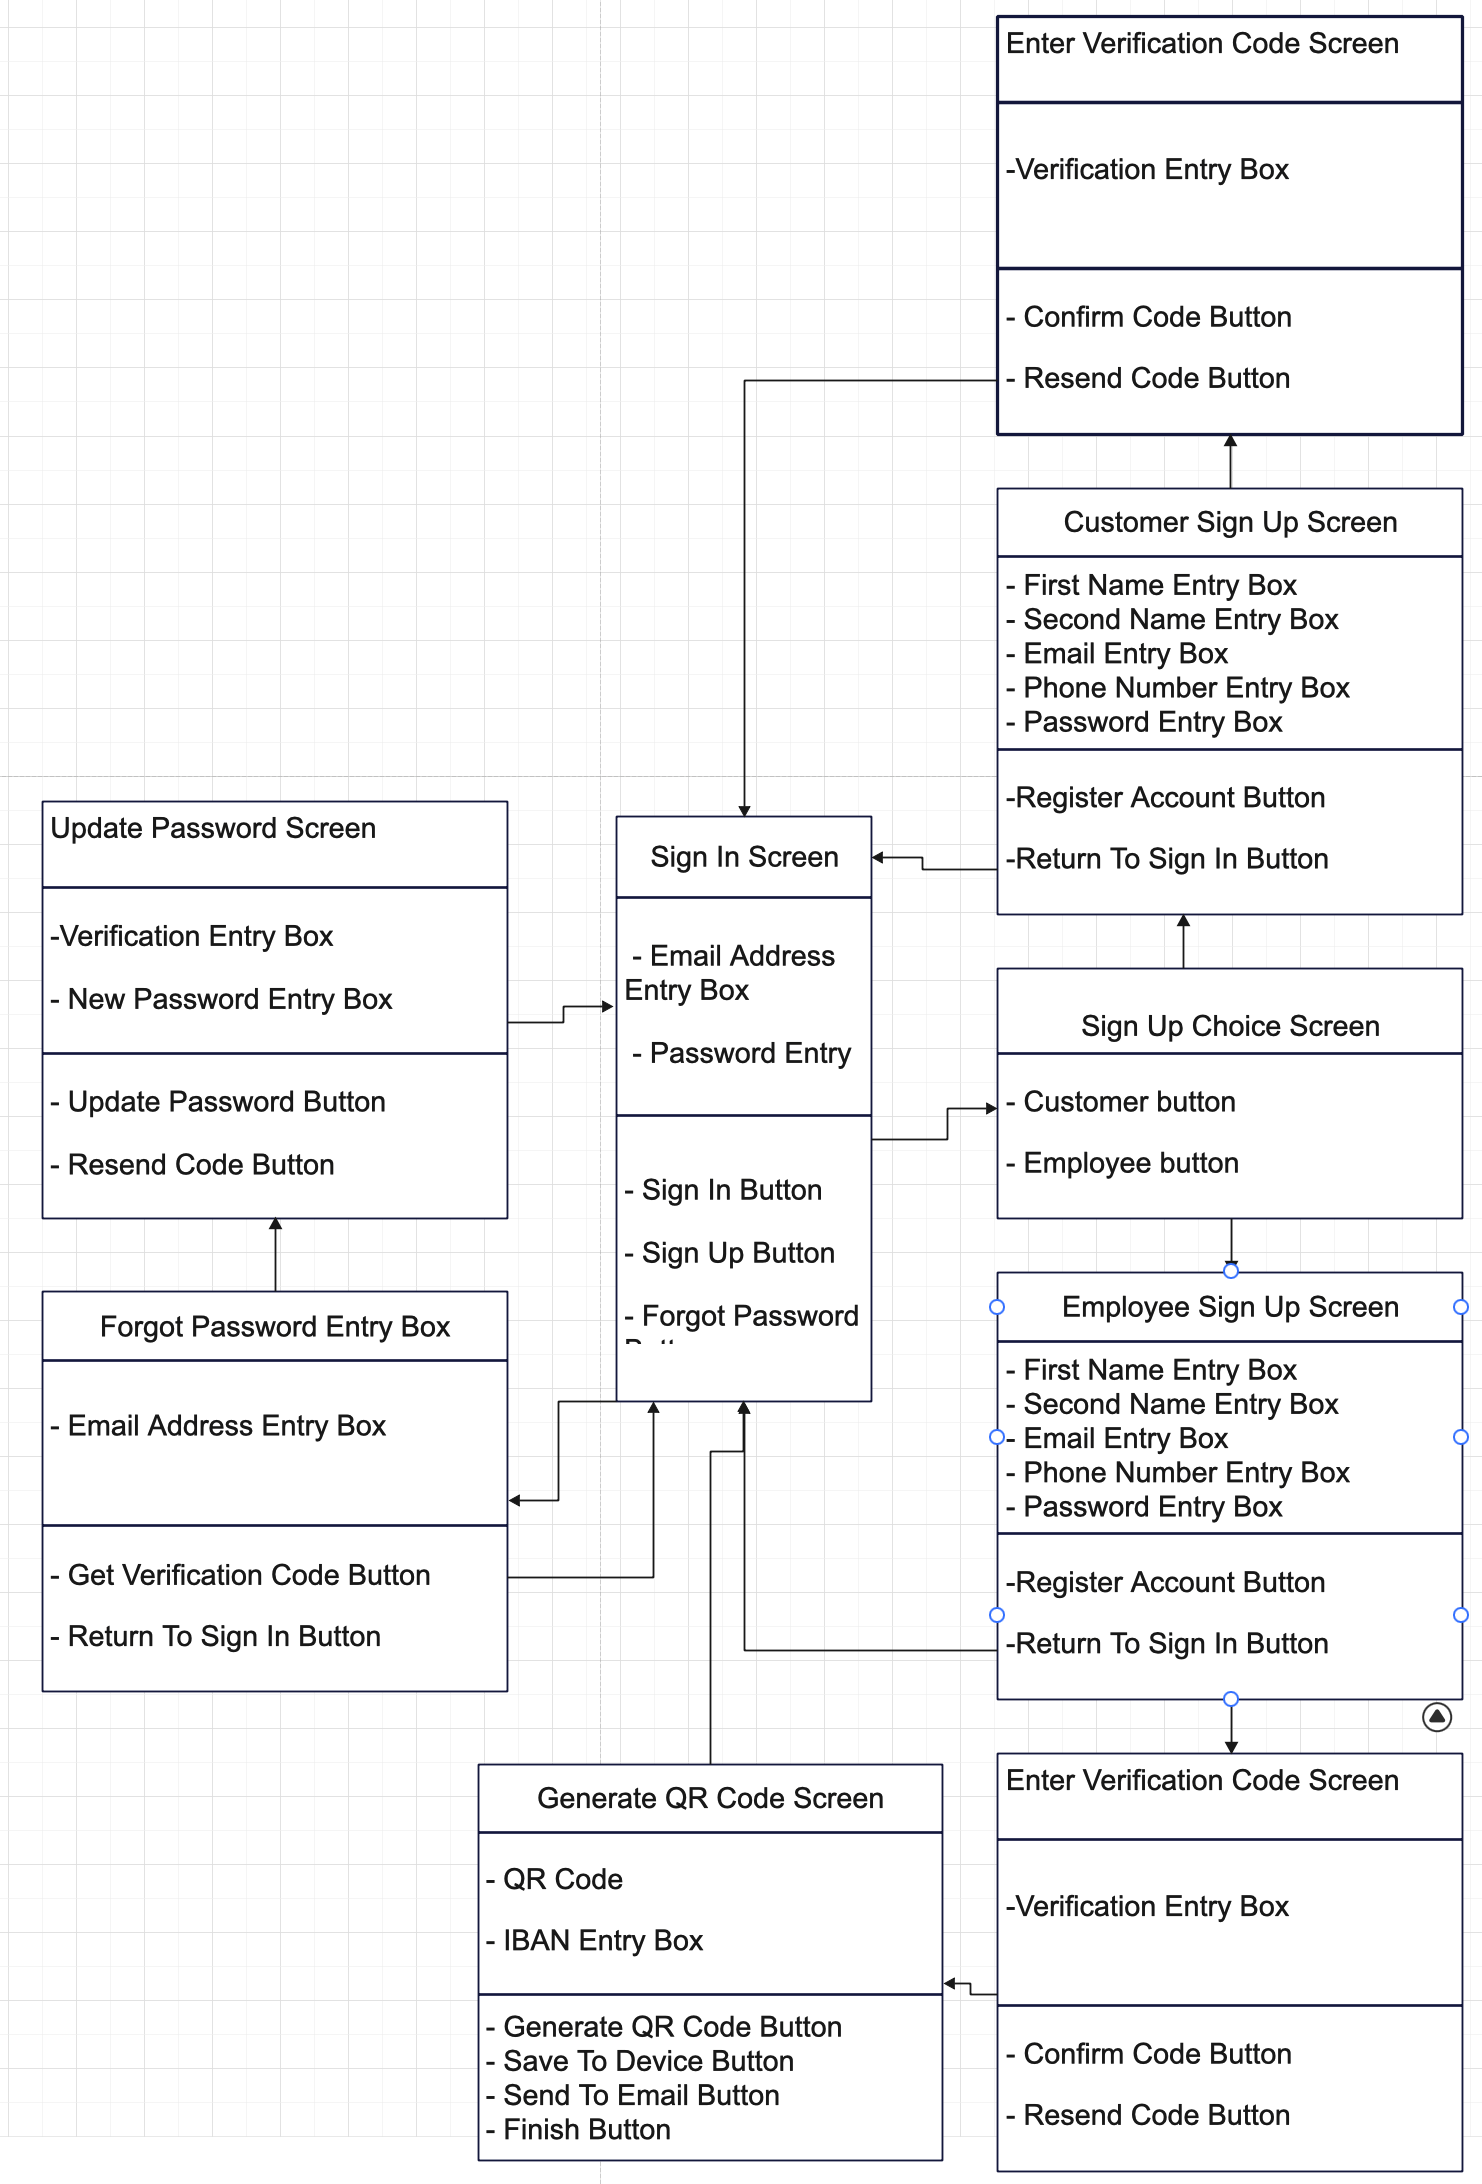
\includegraphics[scale = .40]{atu-computing-latex-template/images/Auth UML.png}
\end{center}

\section{Homepage and updating user details}
When the user logged in they are met with three options. They can either make a tip, updated account details or sign out. To start, if the user wants to update their email address or their password they tap 'Update account details'. If the user does this, they are met with two options, 'Update email' or 'Update password'. Both have a similar flow. The user just needs to enter a new email or password depending on the option they have chosen and tap the button to make the change and is then brought back to the home page again. For the purposes of security, the user must enter their old password along with the new password to update to a new one. The reason for this being added to the application is the user needs a way to update their information after being logged in. It means they don't have to go through the forgot password authentication route.

\begin{center}
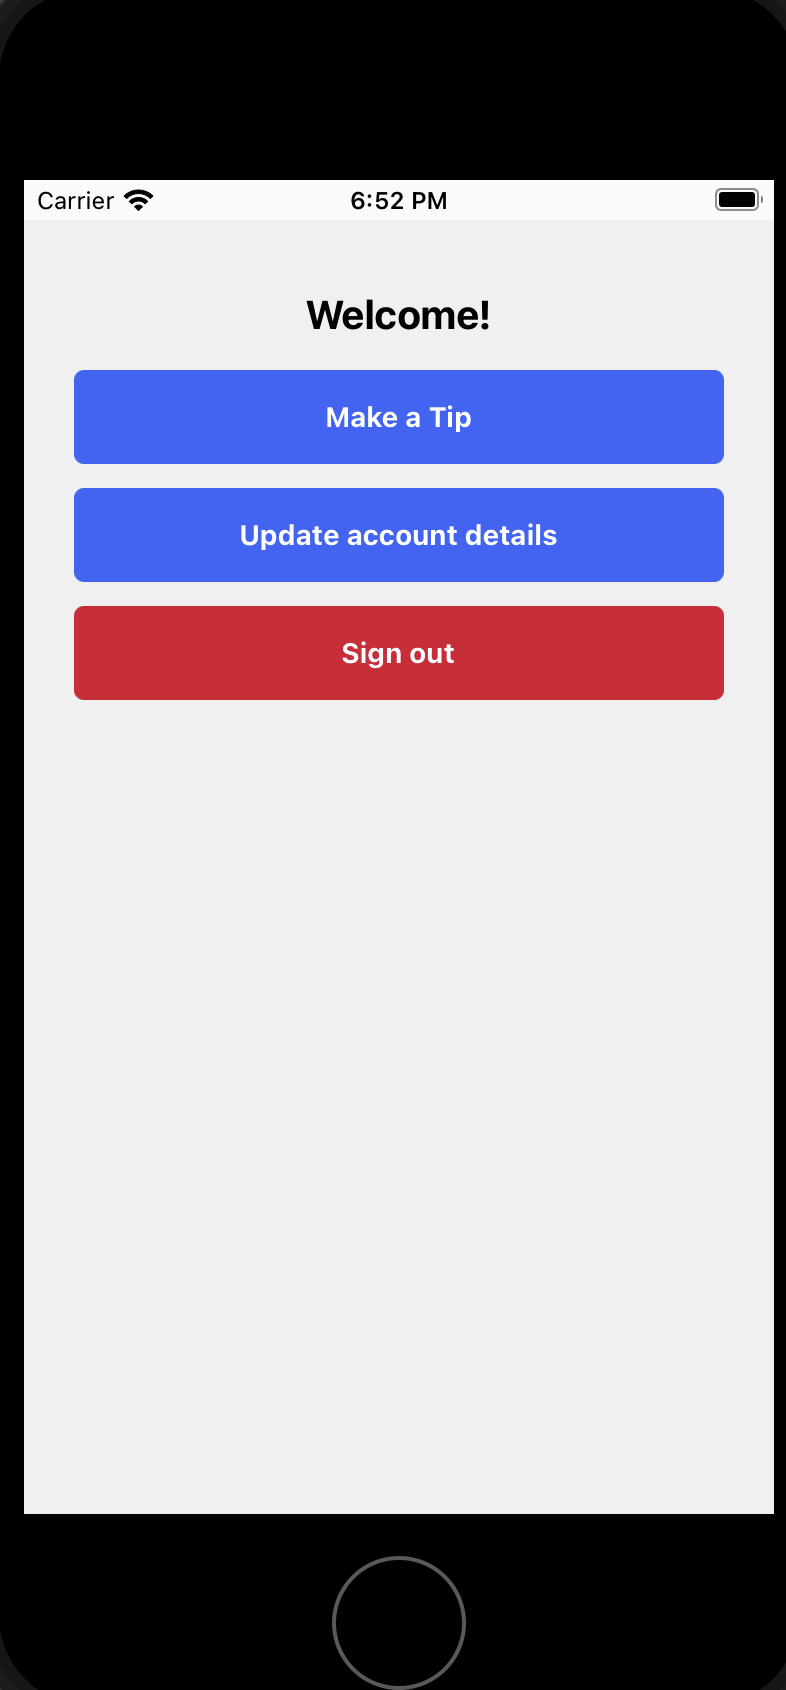
\includegraphics[scale = .40]{atu-computing-latex-template/images/Homepage.png}
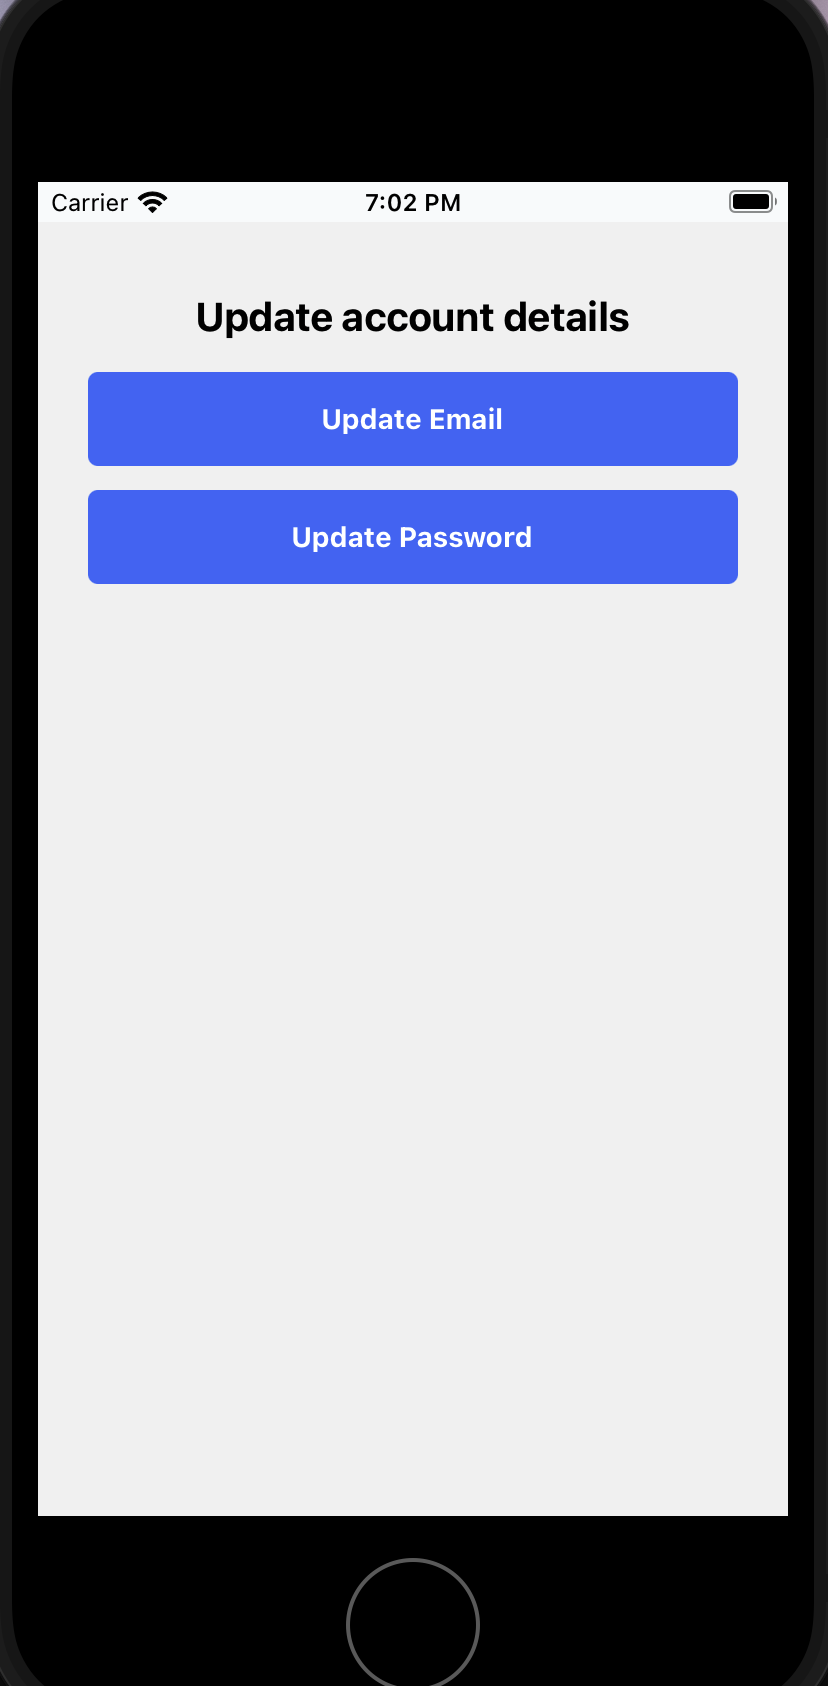
\includegraphics[scale = .40]{atu-computing-latex-template/images/UpdateInfoChoice.png}
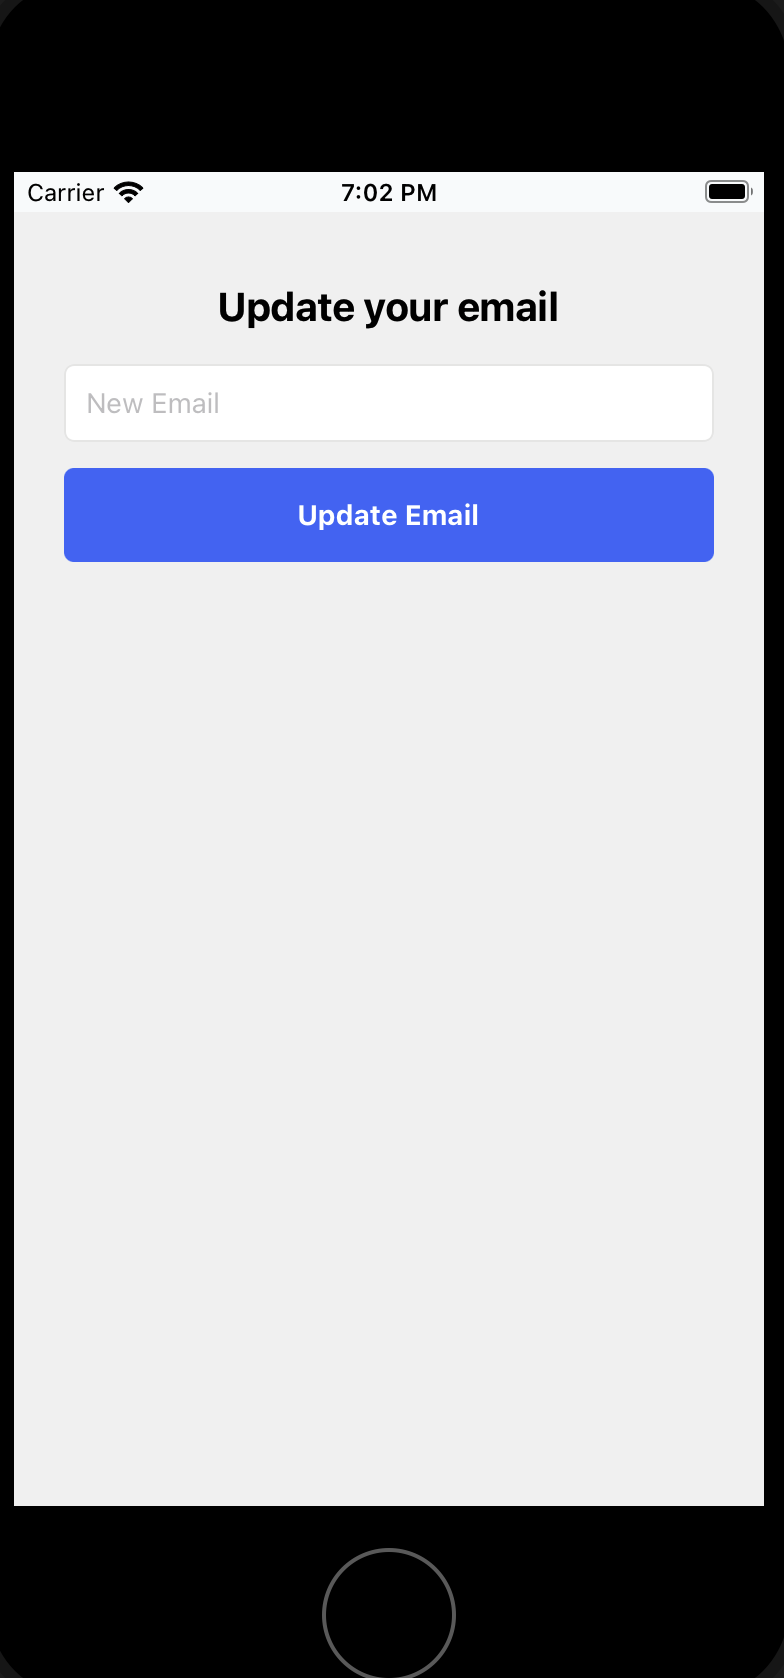
\includegraphics[scale = .40]{atu-computing-latex-template/images/Update email.png}
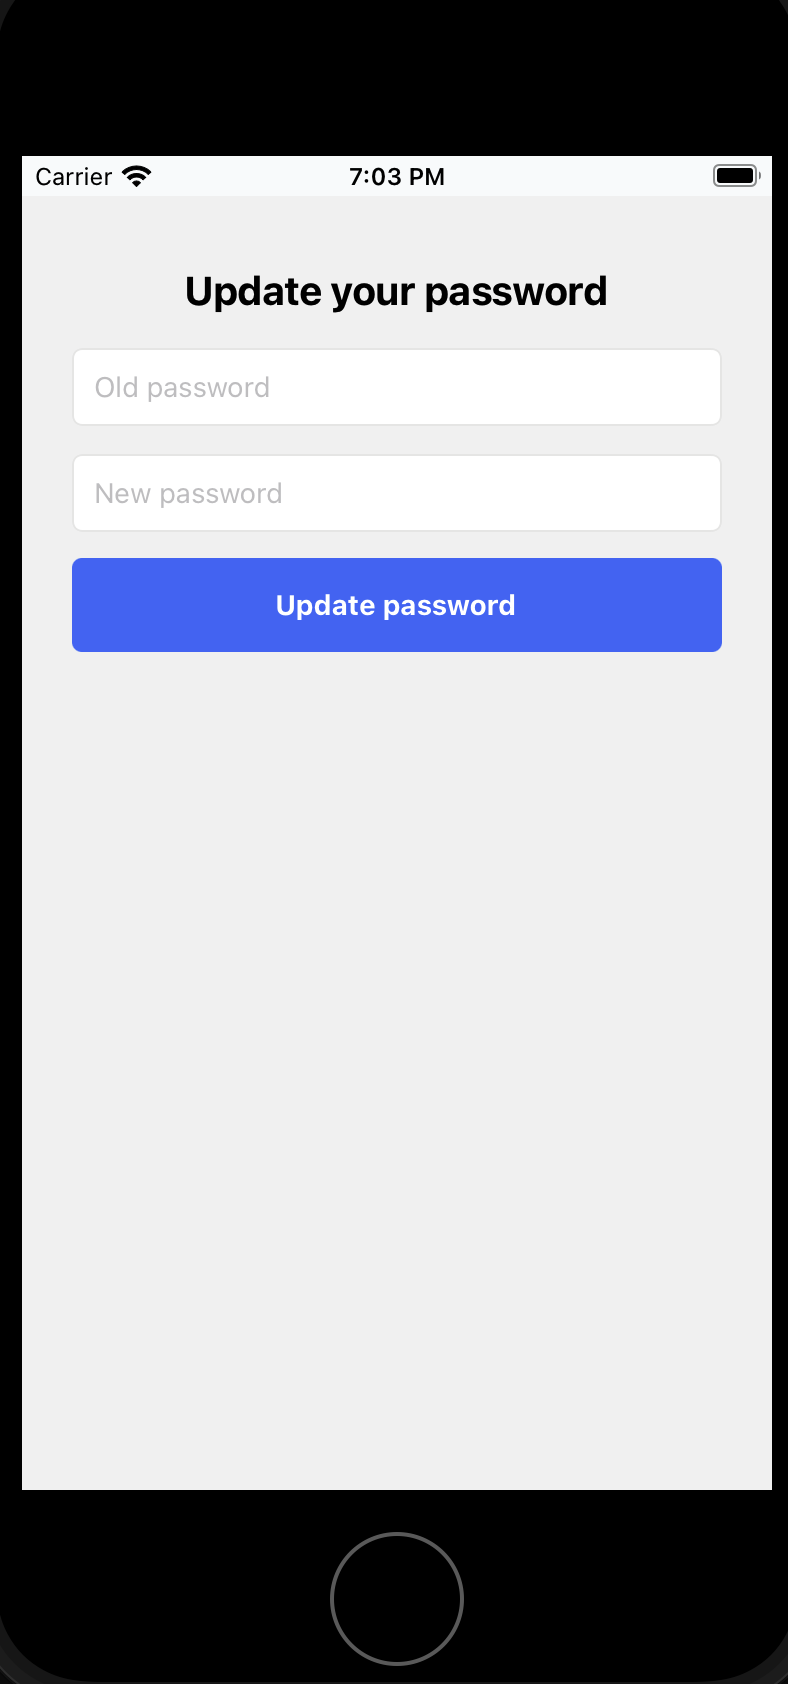
\includegraphics[scale = .40]{atu-computing-latex-template/images/Update password.png}
\end{center}
\section{Tipping  flow}
When the user is on the homepage and decide to make a tip, they tap the Make a Tip button. From there the user is brought to a new screen with two entry boxes, Enter Bill Total and Tip Percentage. After the user has done this, they can tap a button to calculate the tip and they keyboard will disappear. When the user calculates their tip, the calculated tip is presented on screen with a euro symbol beside it. When the user is happy with the amount they would like to tip they tap the Scan QR code button which will open a screen for the user to scan the QR code. If the user has never used the application before, they must give permission to allow camera access. This is what was added to the info.plist file.
\begin{center}
    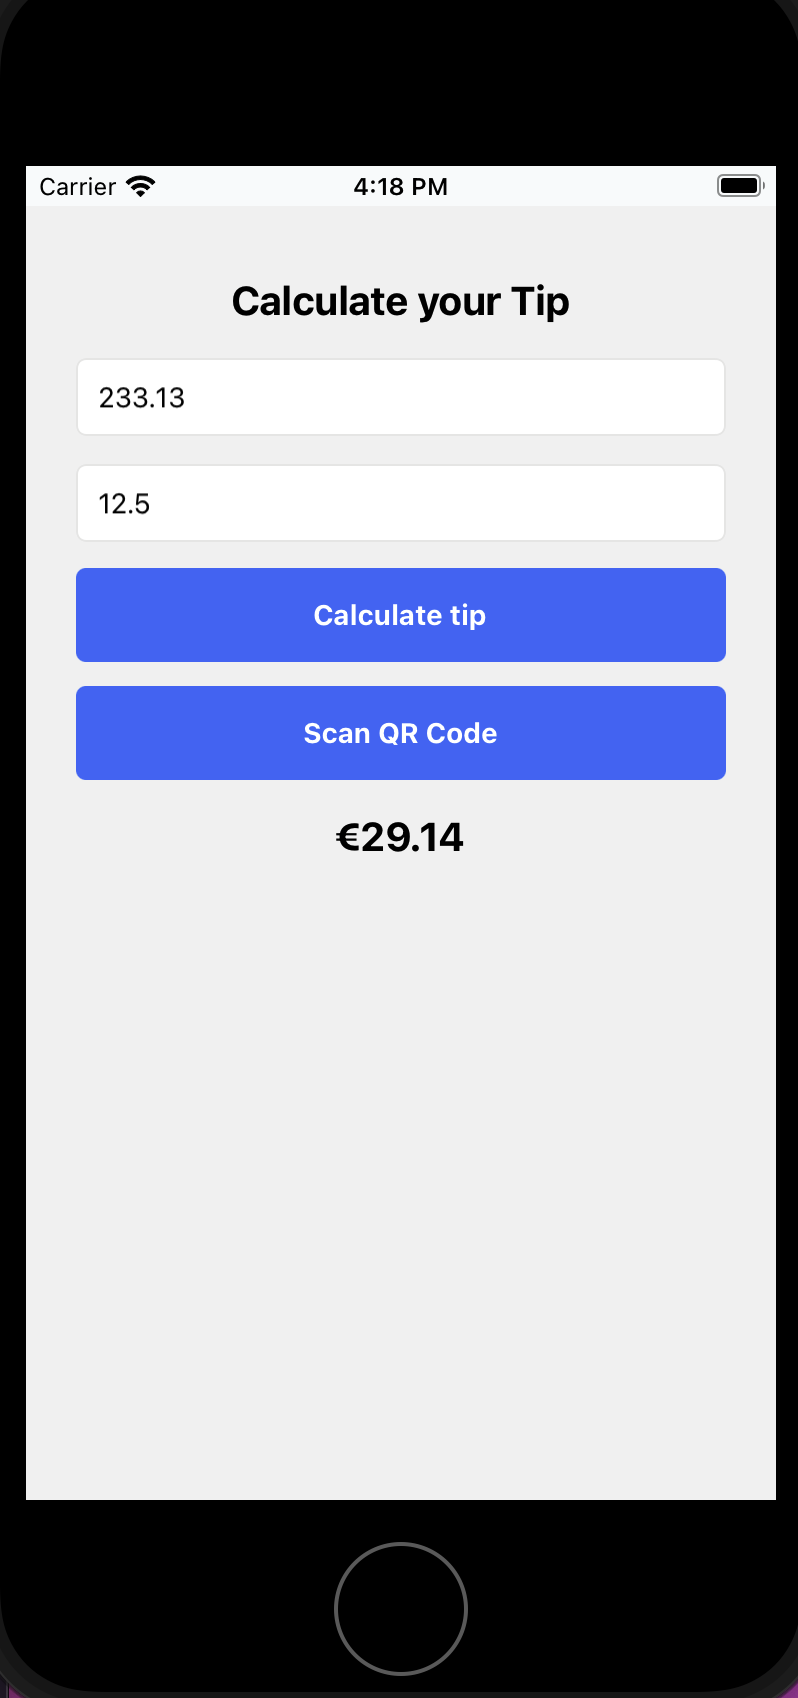
\includegraphics[scale = .40]{atu-computing-latex-template/images/CalculateTip.png}
\end{center}
Once the QR Code has been scanned, the user is brought to the payment screen where they confirm the payment MORE ON THIS
This is the UML diagram for when the user has signed in.
\begin{center}
    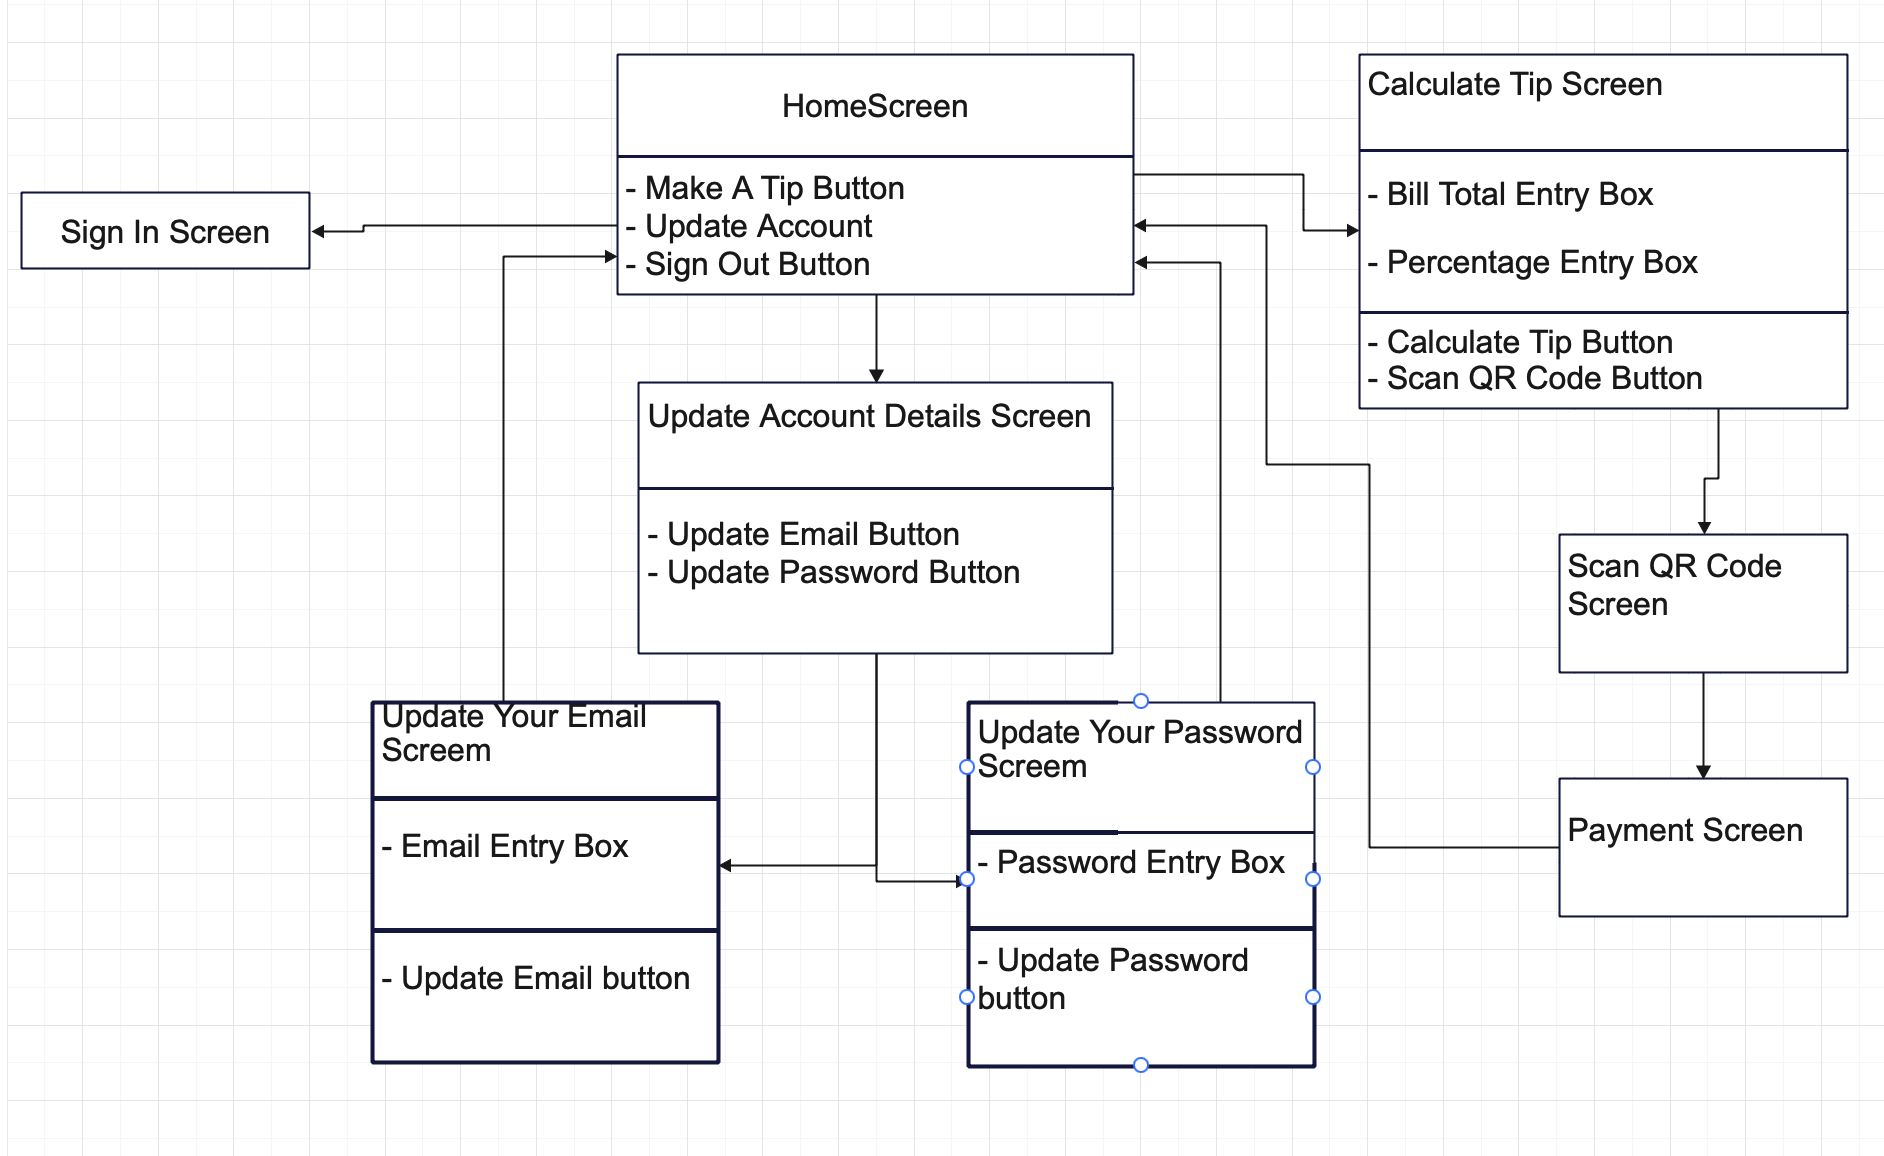
\includegraphics[scale = .40]{atu-computing-latex-template/images/HomeScreen flow.png}
\end{center}
\section{System Architecture}
The architecture is structured like this. First off, we included the MacBook in the diagram as this can depend on whether we are using a physical device or the XCode simulator. So it starts with the MacBook we developed the project on. Next it goes into Visual Studio Code. In there we used React-Native JavaScript which from there we built the application with the command 'react-native run-ios' and then if our iPhone was connected, Tipper was deployed to there or if no device was connected, it was deployed to the simulator through XCode. Next, our app interacted with AWS Amplify on the back-end to handle the login/authentication flow. Finally from the device, it uses Node to create a server that connects to Stripe via a Secret and Public Key to handle the transactions and the user is brought back to the home screen. 
\begin{center}
    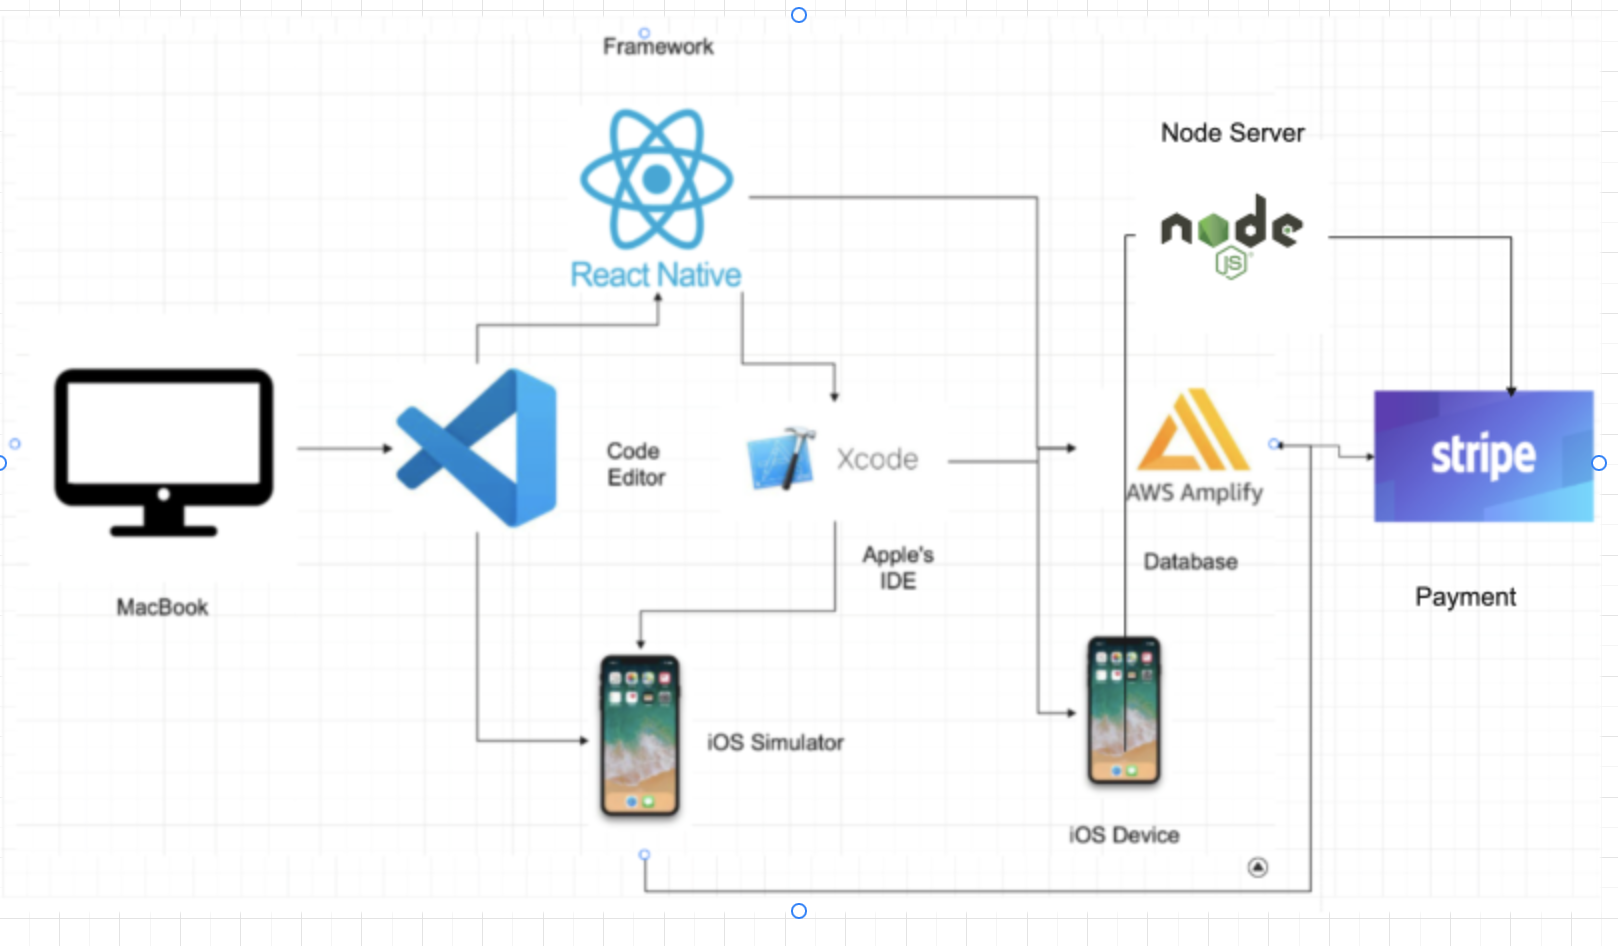
\includegraphics[scale = .55 ]{atu-computing-latex-template/images/SystemArch.png}
\end{center}

